\section{Прогнозное MPC управление}\label{sec:ch3/sec5}

\subsection{Теоретические основы прогнозного MPC управления}\label{subsec:ch3/sec5/sub1}

Метод прогнозного управления (Model Predictive Control, MPC) представляет собой стратегию
оптимального управления с конечным горизонтом прогноза, основанную на итеративном решении задачи оптимизации в
реальном времени. Применительно к электропневматическому приводу с
дискретными распределителями данный метод характеризуется рядом особенностей, обусловленных
спецификой объекта управления и дискретным характером управляющих воздействий.

Фундаментальным принципом прогнозного управления является использование математической модели
объекта для предсказания его поведения на конечном временном горизонте. В общем случае
динамика пневматического привода описывается системой нелинейных дифференциальных уравнений:

\begin{equation}
	\begin{cases}
		\dot{\mathbf{x}}(t) = \mathbf{f}(\mathbf{x}(t), \mathbf{u}(t), \boldsymbol{\theta}) \\
		\mathbf{y}(t) = \mathbf{h}(\mathbf{x}(t))
	\end{cases}
\end{equation}
где $\mathbf{x}(t) \in \mathbb{R}^n$ -- вектор состояния системы, включающий положение $x$ и скорость $v$ штока пневмоцилиндра, массы $m_1$, $m_2$ и температуры $T_1$, $T_2$ воздуха в полостях;
$\mathbf{u}(t) \in \{0,1\}^4$ -- вектор управляющих воздействий, соответствующий состояниям четырех распределителей;
$\boldsymbol{\theta}$ -- вектор параметров модели;
$\mathbf{y}(t) \in \mathbb{R}^p$ -- вектор выходных переменных.

Для реализации алгоритма управления в цифровой форме осуществляется дискретизация модели с периодом квантования $T_s$:

\begin{equation}
	\begin{cases}
		\mathbf{x}_{k+1} = \boldsymbol{\Phi}(\mathbf{x}_k, \mathbf{u}_k, \boldsymbol{\theta}) \\
		\mathbf{y}_k = \mathbf{h}(\mathbf{x}_k)
	\end{cases}
\end{equation}
где $\boldsymbol{\Phi}(\cdot)$ -- дискретное отображение, получаемое численным интегрированием исходной системы на интервале $[kT_s, (k+1)T_s]$.

Принципиальной особенностью рассматриваемой системы является дискретность управляющих воздействий,
что приводит к формулировке задачи смешанного целочисленного программирования на каждом шаге управления:

\begin{equation}
	\begin{aligned}
		\min_{\mathbf{U}_k} \quad & J(\mathbf{U}_k) = \sum_{i=0}^{N_p-1} \ell(\mathbf{x}_{k+i|k}, \mathbf{u}_{k+i|k}) + V_f(\mathbf{x}_{k+N_p|k}) \\
		\text{s.t.} \quad         & \mathbf{x}_{k+i+1|k} = \boldsymbol{\Phi}(\mathbf{x}_{k+i|k}, \mathbf{u}_{k+i|k}, \boldsymbol{\theta})         \\
		                          & \mathbf{u}_{k+i|k} \in \{0,1\}^4                                                                              \\
		                          & \mathbf{x}_{k+i|k} \in \mathcal{X}                                                                            \\
		                          & \mathbf{x}_{k+N_p|k} \in \mathcal{X}_f                                                                        \\
		                          & i = 0,\ldots,N_p-1
	\end{aligned}
\end{equation}
где $\mathbf{U}_k = [\mathbf{u}_{k|k}^T, \ldots, \mathbf{u}_{k+N_p-1|k}^T]^T$ - последовательность управляющих воздействий на горизонте прогноза $N_p$;
$\ell(\cdot)$ - функция стадийных затрат;
$V_f(\cdot)$ - терминальная функция;
$\mathcal{X}$ - множество допустимых состояний;
$\mathcal{X}_f$ - терминальное множество.

Функция стадийных затрат формируется с учетом множественных критериев качества управления:

\begin{equation}
	\ell(\mathbf{x}, \mathbf{u}) = w_1\|\mathbf{y} - \mathbf{r}\|_{\mathbf{Q}}^2 + w_2\|\Delta\mathbf{u}\|_{\mathbf{R}}^2 + w_3\|\mathbf{u}\|_0,
\end{equation}
где $\mathbf{r}$ -- вектор задающих воздействий;
$\|\cdot\|_{\mathbf{Q}}^2$ и $\|\cdot\|_{\mathbf{R}}^2$ -- квадратичные нормы с весовыми матрицами $\mathbf{Q}$ и $\mathbf{R}$;
$\|\cdot\|_0$ -- псевдонорма, подсчитывающая количество переключений;
$w_1$, $w_2$, $w_3$ - весовые коэффициенты.

Существенной проблемой при практической реализации прогнозного управления является наличие параметрических неопределенностей
в модели объекта. Для обеспечения робастности управления применяется минимаксный подход:

\begin{equation}
	\min_{\mathbf{U}_k} \max_{\boldsymbol{\theta} \in \Theta} J(\mathbf{U}_k, \boldsymbol{\theta}),
\end{equation}
где $\Theta$ -- множество возможных значений параметров модели.

Алгоритм прогнозного управления реализуется по принципу отступающего горизонта:

\begin{enumerate}
	\item  В момент времени $k$ измеряется текущее состояние системы $\mathbf{x}_k$;
	\item  Решается задача оптимизации на горизонте $[k, k+N_p]$;
	\item  Реализуется только первое управляющее воздействие $\mathbf{u}_{k|k}$;
	\item  Горизонт прогноза сдвигается на один шаг вперед.

\end{enumerate}

Для учета динамики дискретных распределителей в модель вводятся дополнительные дифференциальные уравнения:

\begin{equation}
	\tau_v\dot{u}_i + u_i = u_{i,cmd}, \quad i = 1,\ldots,4,
\end{equation}
где $\tau_v$ -- постоянная времени распределителя;
$u_{i,cmd}$ -- командный сигнал.

Таким образом, теоретические основы прогнозного управления электропневматическим приводом с дискретными распределителями включают:

\begin{itemize}
	\item Формулировку задачи оптимального управления с учетом дискретности управляющих воздействий;
	\item Построение многокритериальной целевой функции;
	\item Обеспечение робастности к параметрическим неопределенностям;
	\item Гарантирование устойчивости замкнутой системы;
	\item Учет динамики исполнительных устройств.

\end{itemize}
\subsection{Построение прогнозной модели пневмопривода}\label{subsec:ch3/sec5/sub2}

Эффективность прогнозного управления в значительной степени определяется точностью
математической модели объекта управления. При этом модель должна обладать достаточной
простотой для обеспечения вычислительной эффективности алгоритма управления в
реальном времени. В связи с этим предлагается использование редуцированной
модели пневмопривода, сохраняющей основные динамические свойства системы.

Полная термодинамическая модель пневмопривода была представлена в системе \ref{eq:ch2/final_system}. Для применения в
алгоритме прогнозного управления реального времени предлагается её упрощение с использованием следующих допущений:

\begin{enumerate}
	\item Процессы в полостях цилиндра считаются изотермическими $(T_1 = T_2 = T_s)$
	\item Массовый расход через распределители аппроксимируется линейной зависимостью:

	      \begin{equation}
		      G_{ij}(p,u) = k_g u_i (p_u - p_d),
	      \end{equation}
	      где $k_g$ -- коэффициент пропорциональности;
	      $p_u$, $p_d$ -- давления на входе и выходе распределителя соответственно.

	\item Сила трения описывается упрощенной моделью вязкого трения:

	      \begin{equation}
		      F_{\text{тр}}(v) = b v,
	      \end{equation}
	      где $b$ -- коэффициент вязкого трения.
\end{enumerate}

С учетом принятых допущений редуцированная модель принимает вид:
\begin{equation}
	\begin{aligned}
		\dot{x}        & = v                                                                                   \\
		\dot{v}        & = \frac{1}{M}(p_1A_1 - p_2A_2 - (A_1-A_2)p_a - bv)                                    \\
		\dot{p}_1      & = \frac{RT_s}{V_1(x)}(k_g u_1(p_s - p_1) - k_g u_2(p_1 - p_a) - \frac{p_1}{RT_s}A_1v) \\
		\dot{p}_2      & = \frac{RT_s}{V_2(x)}(k_g u_3(p_s - p_2) - k_g u_4(p_2 - p_a) + \frac{p_2}{RT_s}A_2v) \\
		\tau_v\dot{u}i & = -u_i + u{i,cmd}, \quad i = 1,\ldots,4
	\end{aligned}
\end{equation}

Для численной реализации алгоритма прогнозного управления выполняется
дискретизация редуцированной модели методом Рунге-Кутты четвертого порядка:

\begin{equation}
	\mathbf{x}_{k+1} = \mathbf{x}_k + \frac{h}{6}(\mathbf{k}_1 + 2\mathbf{k}_2 + 2\mathbf{k}_3 + \mathbf{k}_4),
\end{equation}
где коэффициенты $\mathbf{k}_i$ вычисляются согласно стандартным формулам метода.

Важным аспектом является оценка точности редуцированной модели. Погрешность
моделирования оценивается путем сравнения с полной термодинамической моделью:

\begin{equation}
	\varepsilon = \sqrt{\frac{1}{N}\sum_{k=1}^N\|\mathbf{x}_k - \mathbf{x}_k^*\|^2}
\end{equation}
где $\mathbf{x}_k^*$ -- состояние полной модели.

Для учета параметрических неопределенностей в модели вводится вектор возмущений:

\begin{equation}
	\mathbf{x}_{k+1} = \boldsymbol{\Phi}(\mathbf{x}_k, \mathbf{u}_k, \boldsymbol{\theta} + \Delta\boldsymbol{\theta})
\end{equation}
где $\Delta\boldsymbol{\theta}$ -- вектор отклонений параметров от номинальных значений, ограниченный множеством:

\begin{equation}
	\Delta\boldsymbol{\theta} \in \mathcal{W} = \{\Delta\boldsymbol{\theta}: \|\Delta\boldsymbol{\theta}\| \leq \delta\}
\end{equation}

Для верификации упрощенной модели было проведено сравнение переходных характеристик с полной термодинамической моделью.

\subsection{Формирование критериев оптимальности и ограничений}\label{subsec:ch3/sec5/sub3}

Эффективность прогнозного управления электропневматическим приводом определяется корректным выбором
критериев оптимальности и формулировкой системы ограничений. Особенностью рассматриваемой задачи является
необходимость учета множественных, зачастую противоречивых,
требований к качеству управления при наличии дискретных управляющих воздействий.

Целевая функция алгоритма прогнозного управления формируется на основе следующих критериев качества:

\begin{enumerate}
	\item Точность позиционирования;
	\item Минимизация количества переключений распределителей;
	\item Энергетическая эффективность;
	\item Быстродействие системы.
\end{enumerate}

Математически задача оптимизации может быть представлена в виде:

\begin{equation}
	J(\mathbf{U}_k) = \sum_{i=0}^{N_p-1} \ell(\mathbf{x}_{k+i|k}, \mathbf{u}_{k+i|k}, \mathbf{r}_{k+i}) + V_f(\mathbf{x}_{k+N_p|k}),
\end{equation}
где функция стадийных затрат $\ell(\cdot)$ включает четыре компонента:

\begin{equation}
	\begin{aligned}
		\ell(\mathbf{x}, \mathbf{u}, \mathbf{r}) = & w_1(x - r)^2 + w_2v^2 +                                    \\
		                                           & + w_3\sum_{i=1}^4|u_i(k) - u_i(k-1)| + w_4\sum_{i=1}^4 u_i
	\end{aligned}
\end{equation}

Здесь первое слагаемое характеризует ошибку позиционирования, второе -- скорость движения, третье -- количество переключений распределителей,
четвертое -- энергопотребление системы. Весовые коэффициенты $w_1$, $w_2$, $w_3$, $w_4$ определяют относительную важность каждого критерия.

Терминальная составляющая $V_f(\cdot)$ вводится для обеспечения устойчивости замкнутой системы:

\begin{equation}
	V_f(\mathbf{x}) = \alpha_1(x - r)^2 + \alpha_2v^2,
\end{equation}
где коэффициенты $\alpha_1$, $\alpha_2$ выбираются из условия убывания функции Ляпунова.

Система ограничений включает:

\begin{enumerate}
	\item Физические ограничения на состояния системы:


	      \begin{equation}
		      \begin{aligned}
			      x_{\min} \leq x \leq x_{\max}        \\
			      p_{\min} \leq p_1, p_2 \leq p_{\max} \\
			      |v| \leq v_{\max}
		      \end{aligned}
	      \end{equation}

	\item Ограничения на управляющие воздействия:

	      \begin{equation}
		      u_i \in \{0,1\}, \quad i = 1,\ldots,4;
	      \end{equation}

	\item Технологические ограничения на частоту переключений:

	      \begin{equation}
		      \sum_{k=1}^{N_p} |u_i(k) - u_i(k-1)| \leq N_{\max}, \quad i = 1,\ldots,4;
	      \end{equation}

	\item Ограничения на минимальное время между переключениями:

	      \begin{equation}
		      t_{k+1} - t_k \geq \Delta t_{\min}.
	      \end{equation}
	      где $t_k$ -- момент $k$-го переключения.
\end{enumerate}

Для обеспечения робастности управления вводятся дополнительные ограничения на запас по давлению:

\begin{equation}
	p_1 - p_2 \geq \Delta p_{\min}.
\end{equation}

Для учета влияния параметрических неопределенностей используется минимаксный подход:

\begin{equation}
	\min_{\mathbf{U}_k} \max_{\boldsymbol{\theta} \in \Theta} J(\mathbf{U}_k, \boldsymbol{\theta}).
\end{equation}

При этом множество $\Theta$ формируется на основе априорной информации о
возможных отклонениях параметров модели от номинальных значений:

\begin{equation}
	\Theta = \{\boldsymbol{\theta}: |\theta_i - \theta_i^*| \leq \Delta\theta_i, i = 1,\ldots,n_{\theta}\}.
\end{equation}

Важным аспектом является выбор весовых коэффициентов целевой функции. Предлагается следующая методика их определения:

\begin{enumerate}
	\item Нормализация каждого компонента целевой функции;
	\item Задание начальных значений весов на основе экспертных оценок;
	\item Корректировка весов по результатам численного моделирования;
	\item Валидация на экспериментальной установке.
\end{enumerate}

Определение оптимальных значений весовых коэффициентов может быть формализовано как задача многокритериальной оптимизации:

\begin{equation}
	\begin{aligned}
		\min_{\mathbf{w}} \quad & \mathbf{F}(\mathbf{w}) = [f_1(\mathbf{w}), f_2(\mathbf{w}), \ldots, f_m(\mathbf{w})]^T \\
		\text{s.t.} \quad       & \sum_{i=1}^4 w_i = 1                                                                   \\
		                        & w_i \geq 0, \quad i = 1,\ldots,4.
	\end{aligned}
\end{equation}

где компоненты вектор-функции $\mathbf{F}(\mathbf{w})$ характеризуют различные показатели качества системы.

Предложенная структура критериев оптимальности и ограничений обеспечивает:

\begin{enumerate}
	\item Высокую точность позиционирования;
	\item Увеличение ресурса пневмораспределителей;
	\item Энергетическую эффективность системы;
	\item Робастность к параметрическим возмущениям;
	\item Выполнение технологических требований.
\end{enumerate}

Эффективность разработанного подхода подтверждается результатами численного моделирования и экспериментальными
исследованиями, представленными в последующих разделах.

\subsection{Алгоритм решения задачи оптимизации в реальном времени}\label{subsec:ch3/sec5/sub4}

Практическая реализация прогнозного управления электропневматическим
приводом с дискретными распределителями требует эффективного алгоритма
решения задачи смешанного целочисленного программирования в реальном времени.
Специфика задачи заключается в необходимости учета дискретности управляющих воздействий и
жестких временных ограничений на процесс оптимизации.

Сформулированная в предыдущем разделе задача оптимизации может быть представлена в обобщенном виде:
\begin{equation}
	\begin{aligned}
		\min_{\mathbf{U}_k} \quad & J(\mathbf{U}_k) = \sum_{i=0}^{N_p-1} \ell(\mathbf{x}_{k+i|k}, \mathbf{u}_{k+i|k}, \mathbf{r}_{k+i}) + V_f(\mathbf{x}_{k+N_p|k}) \\
		\text{s.t.} \quad         & \mathbf{x}_{k+i+1|k} = \boldsymbol{\Phi}(\mathbf{x}_{k+i|k}, \mathbf{u}_{k+i|k})                                                \\
		                          & \mathbf{u}_{k+i|k} \in {0,1}^4                                                                                                  \\
		                          & \mathbf{x}_{k+i|k} \in \mathcal{X}                                                                                              \\
		                          & t_{\text{opt}} \leq T_s
	\end{aligned}
\end{equation}
где $t_{\text{opt}}$ -- время решения задачи оптимизации;
$T_s$ -- период дискретизации системы управления.

Для решения данной задачи предлагается использовать модифицированный метод ветвей
и границ с применением эвристик для ускорения поиска решения. Основные этапы алгоритма включают:

Релаксацию целочисленных ограничений:
\begin{equation}
	\mathbf{u}_{k+i|k} \in [0,1]^4.
\end{equation}

Решение релаксированной задачи методом последовательного квадратичного программирования:
\begin{equation}
	\begin{aligned}
		\mathbf{U}_{k+1} & = \mathbf{U}_k - \alpha_k \mathbf{H}_k^{-1}\nabla J(\mathbf{U}_k) \\
		\mathbf{H}_k     & = \nabla^2 J(\mathbf{U}_k) + \mu_k\mathbf{I}
	\end{aligned}
\end{equation}

Округление полученного решения с учетом предыстории управления:
\begin{equation}
	\hat{u}_i = \begin{cases}
		1, & u_i \geq 0.5 + \delta_i \\
		0, & u_i < 0.5 + \delta_i
	\end{cases}
\end{equation}
где $\delta_i$ -- поправка, учитывающая предыдущие состояния распределителей.

Для ускорения сходимости алгоритма используется схема предварительного прогнозирования состояния системы, представленная
на рисунке \ref{fig:mpc_structure}.

\begin{figure}[ht]
	\centering
	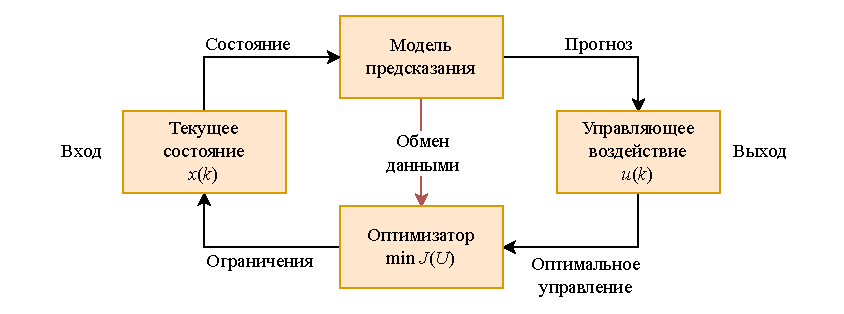
\includegraphics{part3/структура алгоритма прознозного управления.pdf}
	\caption{Структура алгоритма прогнозного управления}\label{fig:mpc_structure}
\end{figure}

Для оценки вычислительной эффективности предложенного алгоритма введем метрику времени решения задачи
оптимизации, результаты анализа показаны на рисунке \ref{fig:opt_compar}а.

Статистический анализ показывает, что в 95\% случаев время решения задачи
оптимизации не превышает 3 мс при периоде дискретизации системы управления
10 мс, что обеспечивает возможность работы алгоритма в реальном времени.

Для повышения робастности алгоритма используется адаптивная схема определения
параметров оптимизации:

\begin{equation}
	\begin{aligned}
		\mu_k    & = \beta|\nabla J(\mathbf{U}_k)| \\
		\alpha_k & = \frac{\gamma}{|\mathbf{H}_k|} \\
		\delta_i & = \lambda(u_i(k-1) - 0.5)
	\end{aligned}
\end{equation}
где $\beta$, $\gamma$, $\lambda$ -- настроечные коэффициенты.

Эффективность предложенного алгоритма подтверждается результатами численного моделирования, представленных на рисунке \ref{fig:opt_compar}б.

\begin{figure}[ht]
	\centering
	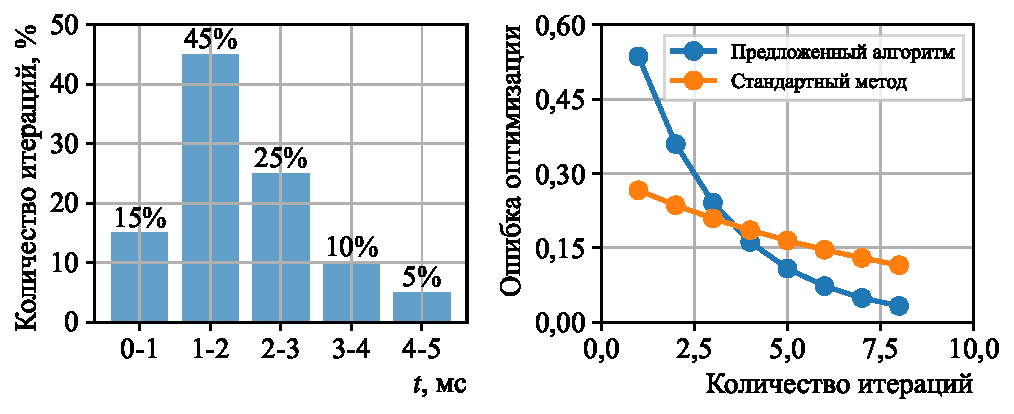
\includegraphics{part3/optimization_comparison.pdf}
	\caption{Зависимость времени решения задачи оптимизации от горизонта прогноза}\label{fig:opt_compar}
\end{figure}